\documentclass[9pt,a4paper]{article} % use larger type; default would be 10pt
\NeedsTeXFormat{LaTeX2e}
\makeindex

%---------------------------- PACKAGE INCLUSION -------------------------------
% This group renders characters clearer and more precise

\RequirePackage[bitstream-charter,cal,expert]{mathdesign}
\RequirePackage{charter}
\RequirePackage{helvet}
\RequirePackage{makeidx}
\RequirePackage{latexsym}

\usepackage{geometry}
\geometry{a4paper,
		  top=4em,
		  left=3em,
		  right=3em,
		  bottom=3.39em
		  }

\usepackage{array,multirow,booktabs}
\usepackage{graphicx}
\usepackage{adjustbox}
\usepackage{xspace}
\usepackage[parfill]{parskip} % Activate to begin paragraphs with an empty line rather than an indent
\usepackage{paralist} % very flexible & customisable lists (eg. enumerate/itemize, etc.)
\usepackage{listings} % for lstset definitions
\usepackage{url}
\usepackage{subfig} % make it possible to include more than one captioned figure/table in a single float
\usepackage{epsfig}
\usepackage{gensymb}
\usepackage{textcomp}
\usepackage{booktabs}

\usepackage{amsmath}
\newcommand{\mathbold}[1]{\text{\textbf{#1}}}

\usepackage{xcolor}
\definecolor{yerothColorOrange}{RGB}{242, 161, 0}   
\definecolor{yerothColorBlue}{RGB}{77 , 93 , 254}
\definecolor{yerothColorRed}{RGB}{254, 48 , 48}
\definecolor{yerothColorGray}{RGB}{198, 198, 198}
\definecolor{yerothColorDarkgray}{RGB}{60, 60 , 60}
\definecolor{yerothColorIndigo}{RGB}{83, 0, 125}
\definecolor{yerothColorGreen}{RGB}{2  , 160, 70}
\definecolor{forestgreen}{RGB}{2,160,70}    
\definecolor{mediumblue}{RGB}{7,43,205}    
\definecolor{firebrickred}{RGB}{178,34,34}
\definecolor{listingray}{gray}{0.9}
\definecolor{lbcolor}{rgb}{0.9,0.9,0.9}
\definecolor{darkgreen}{rgb}{0,0.35,0}
\definecolor{medgreen}{rgb}{0,0.5,0}
\definecolor{lightgreen}{rgb}{0.5,0.7,0.5}
\definecolor{pmcolour}{rgb}{0.5,0.7,0.5}
\definecolor{medgrey}{rgb}{0.6,0.6,0.6}
\definecolor{purplish}{rgb}{0.4,0,0.6}
\definecolor{brightred}{rgb}{1,0.2,0.2}


\newcommand{\yerothrdCOLOR}{\textcolor{yerothColorGreen}
			{\textsc{\textcolor{yerothColorRed}{YEROTH}}$_{\text{r\&d}}$\xspace}}

\newcommand{\yerothrd}{YEROTH~R\&D\xspace}

\newcommand{\myfullacademicname}{PR. XAVIER NOUMBISSI NOUNDOU\xspace}


\usepackage{hyperref}
\hypersetup{
    colorlinks,
    pagebackref,
    citecolor=medgreen,
    linkcolor=purplish,
    breaklinks,
    pdftex,
    bookmarks,
    plainpages=false,
    pdftitle={CURRICULUM VITAE DU PROFESSEUR PLEIN (\yerothrd) XAVIER NOUMBISSI NOUNDOU.},
    pdfauthor={PR. XAVIER NOUMBISSI NOUNDOU (@\yerothrd)}
}

% format two pieces of text, one left aligned and one right aligned
\newcommand{\headerrow}[2]
{\begin{tabular*}{\linewidth}{l@{\extracolsep{\fill}}r}
	#1 &
	#2 \\
\end{tabular*}}

\newcommand{\headerrowONE}[1]{\headerrow{#1}{}}

\newcommand{\emphbold}[1]{\textbf{\emph{#1}}\xspace}

\newcommand{\git}{Git\xspace}

\newcommand{\yerothitem}[1]
{
	\item 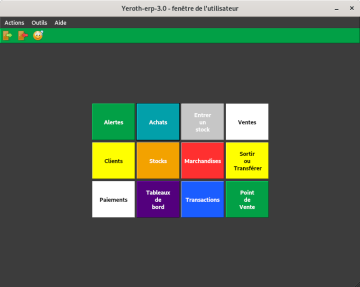
\includegraphics[scale=0.03]{yeroth-erp-3-0.png} #1
}

\newcommand{\yerothUNIBREMENitem}[1]
{
	\item 
\includegraphics[scale=0.05]{YEROTH-LOGO-UNI-BREMEN-2021.png} #1
}


\newcommand{\yerothUWATERLOOWATFORMitem}[1]
{
	\item 
\includegraphics[scale=0.07]{YEROTH-LOGO-UWATERLOO-WATFORM.jpg} #1
}

\newcommand{\yerothpgitroispointzero}{YEROTH--PGI--$3$.$0$\xspace}

\newcommand{\cplusplus}{C$++$\xspace}
\newcommand{\java}{\texttt{Java}\xspace}

\newcommand{\css}{\texttt{CSS}\xspace}
\newcommand{\html}{\texttt{HTML$5$}\xspace}
\newcommand{\jtwoee}{J$2$EE\xspace}
\newcommand{\php}{\texttt{PHP}\xspace}

\newcommand{\dpkgmanager}{\texttt{dpkg (debian package manager)}\xspace}
\newcommand{\innosetuppackagemanager}{\texttt{Inno Setup package manager (pour MS~WINDOWS)}\xspace}

\newcommand{\AWK}{\texttt{AWK}\xspace}
\newcommand{\bash}{\texttt{BASH}\xspace}
\newcommand{\python}{\texttt{Python}\xspace}

\newcommand{\scala}{\texttt{Scala}\xspace}
\newcommand{\haskell}{\texttt{Haskell}\xspace}
\newcommand{\ml}{\texttt{ML}\xspace}

\newcommand{\mysql}{\texttt{MySQL}\xspace}
\newcommand{\sqlite}{\texttt{SQLite}\xspace}

\newcommand{\yerothdebian}{\texttt{DEBIAN LINUX}\xspace}
\newcommand{\ms}{\texttt{Windows~XP, $2000$}\xspace}
\newcommand{\redhat}{\texttt{RedHat~linux}\xspace}

\newcommand{\cvitemdate}[2]{#1~$#2$\xspace}
\newcommand{\cvitempositionheld}[1]{\textbf{#1}\xspace}

%%%%%%%%%%%%%%%%%%%%SETTING HEADER AND FOOTER FOR 'REPORT CLASS'.%%%%%%%%%%%%%%%%%%%%%
\usepackage{lastpage}
\usepackage{fancyhdr}
\pagestyle{fancy}
\renewcommand{\headrulewidth}{0pt}
\fancyhf{}

\fancypagestyle{plain}{% copies "fancy" over "plain"
  \fancyfoot[C]{\thepage}% you can add edits that won't affect "fancy" but only "plain"
}

\fancypagestyle{OnlyFirstPage}{%
	\lhead{YEROTH R\&D}
	\rhead{\url{http://sites.google.com/view/yeroth-rd}}
    \lfoot{}
}

\rhead{\url{http://sites.google.com/view/yeroth-rd}}
\lhead{YEROTH R\&D}
\lfoot{}
\rfoot{}
%\cfoot{\thepage}

\renewcommand{\headrulewidth}{0pt}

%\pagenumbering{gobble}
\cfoot{\thepage\ DE \pageref{LastPage}}


\begin{document}

\thispagestyle{OnlyFirstPage}

\bigskip


\headerrow{\Large \textbf{\myfullacademicname}}
{\Large \textbf{yeroth.rd.30@gmail.com}}

\vspace{1em}


\hrule
\begin{center}
{\large \textbf{PARCOURS ACADÉMIQUE}}
\end{center}

\vspace{0.5em}

\headerrowONE{\textbf{Doctor of Philosophy in Computer Engineering (''Doctorat/Ph.D en Génie informatique'')}}	
\headerrowONE{\href{http://watform.uwaterloo.ca/}{WatForm Lab, Université de Waterloo, Waterloo, Ontario, CANADA}}
\headerrowONE{\href{http://archive.org/download/yeroth-saint/YEROTH-SAINT.PDF}{Ph.D.~Thesis: Context-Sensitive Staged Static Taint Analysis for C using LLVM}}
\headerrowONE{\cvitemdate{Octobre}{2009} -- \cvitemdate{Mars}{2015} (abandon avec $1$ MOYENNE DE $17.50~/~20$)}	
	
\vspace{0.3em}
	
\headerrowONE{\href{http://www.informatik.uni-bremen.de/agbs/qualifikationsarbeiten/diplomarbeiten_e.html}{\textbf{Diplom--Informatiker (Dipl.--Inf. ou encore ''Diplôme de Master II en Génie informatique'')}}}
\headerrowONE{\href{http://www.informatik.uni-bremen.de/agbs/}{AGBS, Université de Brême, Brême, Bremen, ALLEMAGNE}}	
\headerrowONE{Master's degree Thesis: Statistical test case generation for reactive systems}
\headerrowONE{\cvitemdate{$01$~Octobre}{2002} -- \cvitemdate{$25$~Mai}{2007} (succès avec $1$ MOYENNE DE $17.50~/~20$)}	

\vspace{1em}
%%%%%%%%%%%%%%%%%%%%%%%%%%%%%%%%%%%%%%%%%%%%%%%%%%%%%%%%%%%%%%%%%%%%%%

\hrule
\begin{center}
{\large \textbf{INVENTIONS EN GÉNIE INFORMATIQUE}}
\end{center}

\vspace{0.5em}

\headerrowONE{\href{http://archive.org/download/yeroth-erp-3-0-info-francais/yeroth-erp-3-0-info-francais.pdf}{\textbf{PGI (PROGICIEL DE GESTION INTÉGRÉ) '\texttt{YEROTH--PGI--3.0--STANDALONE}'}}}		
\headerrowONE{\cvitemdate{Octobre}{2015} -- En cours}
\headerrowONE{Code source libre et gratuit: \url{http://github.com/xnoumbissinoundou/yeroth-erp-3.0}}

\vspace{0.3em}

\headerrowONE{\textbf{'YEROTH-PGI-3.0--SYSTEM--DAEMON': ALERTES ET SAUVEGARDE AUTOMATISÉE}
  POUR \textbf{'\texttt{YEROTH--PGI--3.0--STANDALONE}'}}
  \headerrowONE{\cvitemdate{Octobre}{2015} -- En cours}
\headerrowONE{Code source libre et gratuit: \url{http://github.com/xnoumbissinoundou/yeroth-erp-3.0-system-daemon}}

\vspace{0.3em}

\headerrowONE{\textbf{SCRIPTS DE DÉVELOPPEMENT ET D'INSTALLATION
  POUR 
  \href{http://github.com/xnoumbissinoundou/yeroth-erp-3.0}{\textbf{YEROTH--PGI--3.0--STANDALONE}}}}
  \headerrowONE{\cvitemdate{Octobre}{2015} -- En cours}
\headerrowONE{Code source libre et gratuit: \url{http://github.com/xnoumbissinoundou/yeroth-rd-binaries-folder-scripts}}

\vspace{0.3em}

\headerrowONE{\href{http://archive.org/download/yeroth-saint/YEROTH-SAINT.PDF}{\textbf{CONTEXT-SENSITIVE STAGED STATIC TAINT ANALYSIS FOR C USING LLVM (\texttt{'YEROTH--SAINT'})}}}
\headerrowONE{\cvitemdate{Octobre}{2009} -- \cvitemdate{Octobre}{2015}}
\headerrowONE{Code source libre et gratuit: \url{http://github.com/xnoumbissinoundou/yeroth.rd.saint}}
	
	
\vspace{1em}
%%%%%%%%%%%%%%%%%%%%%%%%%%%%%%%%%%%%%%%%%%%%%%%%%%%%%%%%%%%%%%%%%%%%%%


\hrule
\begin{center}
{\large \textbf{EXPÉRIENCE PROFESSIONNELLE}}
\end{center}

\vspace{0.5em}

\headerrowONE{\textbf{\yerothrd, Douala, LITTORAL, CAMEROUN}}
\headerrowONE{\cvitempositionheld{PROFESSEUR DE RECHERCHE en génie informatique, CEO}}
\headerrowONE{\cvitemdate{Octobre}{2015} -- Présent}	

\vspace{0.3em}

\headerrowONE{\textbf{WatForm Lab, Université de Waterloo, Waterloo, ON, CANADA}}	
\headerrowONE{\cvitempositionheld{ASSISTANT D'ENSEIGNEMENT}}
\headerrowONE{\cvitemdate{Octobre}{2009} -- \cvitemdate{Mars}{2015}}
	
\vspace{0.3em}

\headerrowONE{\textbf{IBM Toronto Software Lab, Markham, ON, CANADA}}	
\headerrowONE{\cvitempositionheld{DÉVELOPPEUR LOGICIEL \cplusplus} (optimisation de la compilation JAVA--JIT--J$9$
	pour IBM WEBSPHERE), DOCTORANT/PH.D.}
\headerrowONE{\cvitemdate{Janvier}{2012} -- \cvitemdate{Août}{2012}}	

\vspace{0.3em}

\headerrowONE{\textbf{SIEMENS Medical Solutions, Erlangen, Bavière, ALLEMAGNE}}	
\headerrowONE{\cvitempositionheld{DÉVELOPPEUR LOGICIEL JUNIOR \cplusplus} (protocole 
de communication '\texttt{DMIP}' pour la radiothérapie avec '\texttt{LINAC}--Siemens')}
\headerrowONE{\cvitemdate{Novembre}{2007} -- \cvitemdate{Juillet}{2009}}	
	
\vspace{0.3em}

\headerrowONE{\textbf{Greenpeace e.V, Hambourg, Hambourg, ALLEMAGNE}}	
\headerrowONE{\cvitempositionheld{TESTEUR MANUEL DE LOGICIEL} 
(logiciel '\texttt{MOVE}' développé par la société '\texttt{sd\&m}' pour la gestion de Greenpeace e.V)}
\headerrowONE{\cvitemdate{Mars}{2007} -- \cvitemdate{Avril}{2007}}	

\vspace{0.3em}

\headerrowONE{\textbf{Bergmann Automaten GmbH, Rellingen, Hambourg, ALLEMAGNE}}	
\headerrowONE{\cvitempositionheld{DÉVELOPPEUR LOGICIEL} \cplusplus, \jtwoee (protocoles de
communication (ex.: '\texttt{SIPv$2$}'), serveurs '\texttt{JAVA-servlets}'\\
 pour automates de payements dans des mairies ou libraries en ALLEMAGNE)}
\headerrowONE{\cvitemdate{Avril}{2005} -- \cvitemdate{Avril}{2007}}	
	
\vspace{0.3em}

\headerrowONE{\textbf{AGBS--Université de Brême, Brême, Brême, ALLEMAGNE}}	
\headerrowONE{\href{http://www.informatik.uni-bremen.de/agbs/jp/papers/peleska_et_al_soqua2006.pdf}
	{\cvitempositionheld{DÉVÉLOPPEUR LOGICIEL \cplusplus}} (plugin de 
génération de classes \cplusplus modélisant des 'statecharts (\texttt{UML})', '\texttt{Borland-Together}')}
\headerrowONE{\cvitemdate{Septembre}{2006} -- \cvitemdate{Février}{2007}}	

\vspace{0.3em}

\headerrowONE{\textbf{We$4$IT GmbH, Brême, Brême, ALLEMAGNE}}	
\headerrowONE{\cvitempositionheld{STAGIAIRE--DÉVELOPPEUR LOGICIEL} \mysql, \jtwoee
(application web pour gestion des formations du personnel hospitalier)}
\headerrowONE{\cvitemdate{Juin}{2005} -- \cvitemdate{Juillet}{2005}}

\vspace{0.3em}

\headerrowONE{\textbf{bremen$4$u GmbH, Brême, Brême, ALLEMAGNE}}	
\headerrowONE{\cvitempositionheld{STAGIAIRE--DÉVELOPPEUR WEB, ADMINISTRATION--SYSTÈME} \mysql, \redhat, \php,
\html, \css}
\headerrowONE{\cvitemdate{Mars}{2004}}	
	
\vspace{0.3em}

\headerrowONE{\textbf{ZMML--Université de Brême, Brême, Brême, ALLEMAGNE}}	
\headerrowONE{\cvitempositionheld{DÉVELOPPEUR WEB} \html, \css (programmation de pages web,
et de tests d'évaluations pour étudiants avec le RAD--SERVER)}
\headerrowONE{\cvitemdate{Février}{2003} -- \cvitemdate{Mars}{2005}}	

\vspace{1em}

%%%%%%%%%%%%%%%%%%%%%%%%%%%%%%%%%%%%%%%%%%%%%%%%%%%%%%%%%%%%

\hrule
\begin{center}
{\large \textbf{PARTICIPATIONS AUX CONFÉRENCES INTERNATIONALES}}
\end{center}

\vspace{0.5em}

\begin{enumerate}
	\item \textbf{PLDI (PROGRAMMING LANGUAGES DESIGN AND IMPLEMENTATION)},
		\cvitemdate{SEPTEMBRE}{2009}, TORONTO, ON, CANADA

	\item \textbf{PLDI (PROGRAMMING LANGUAGES DESIGN AND IMPLEMENTATION)},
		\cvitemdate{SEPTEMBRE}{2013}, TORONTO, ON, CANADA

\end{enumerate}

\vspace{1em}

%%%%%%%%%%%%%%%%%%%%%%%%%%%%%%%%%%%%%%%%%%%%%%%%%%%%%%%%%%%%

\hrule
\begin{center}
{\large \textbf{PARTICIPATIONS AUX ÉCOLES D'ÉTÉ}}
\end{center}

\vspace{0.5em}

\begin{enumerate}
	\item \headerrowONE{\href{http://fm.csl.sri.com/SSFT11/}{\textbf{NATIONAL SCIENCE FOUNDATION, SRI INTERNATIONAL, First Summer School on Formal Techniques},}}
			\headerrowONE{\href{http://fm.csl.sri.com/SSFT11}{\ \hfill  MENLO COLLEGE, ATHERTON, 
			CALIFORNIA, USA (\cvitemdate{$22$ Mai}{2011} -- \cvitemdate{$27$ Mai}{2011})}}

\end{enumerate}

\vspace{1em}

%%%%%%%%%%%%%%%%%%%%%%%%%%%%%%%%%%%%%%%%%%%%%%%%%%%%%%%%%%%%
\hrule
\begin{center}
{\large \textbf{EXPÉRIENCE D'UNITÉS D'ENSEIGNEMENT}}
\end{center}

\vspace{0.5em}

\headerrowONE{\href{http://ece.uwaterloo.ca}{\textbf{UNIVERSITÉ DE WATERLOO}, WATERLOO, ON, CANADA (Octobre~$2009$ -- Mars~$2015$)}}

\begin{enumerate}
	\itemsep -0.3em
	\item COMPILATEURS (DEREK RAYSIDE, Ph.D. (\textbf{MIT, BOSTON, USA}))
	\item PROGRAMMATION DE RÉSEAUX D'ORDINATEURS (MAHESH TRIPUNITARA, Ph.D. (\textbf{PURDUE UNIVERSITY, PURDUE, USA}))
	\item FONDATIONS DU GÉNIE LOGICIEL (IGOR IVKOVIC, Ph.D. (\textbf{UWATERLOO, ON, CANADA}), 
		de regrété mémoire depuis Novembre~$2020$)
	\item MÉTHODES ET OUTILS DE GÉNIE LOGICIEL (IGOR IVKOVIC, Ph.D. (\textbf{UWATERLOO, ON, CANADA}), 
		de regrété mémoire depuis Novembre~$2020$)
	\item PROGRAMMATION POUR PERFORMANCES DE CALCUL (PATRICK LAM, Ph.D. (\textbf{MIT, BOSTON, USA}))
	\item TEST DU LOGICIEL, ASSURANCE QUALITÉ ET MAINTENANCE (PATRICK LAM, Ph.D. (\textbf{MIT, BOSTON, USA}))
\end{enumerate}


\vspace{1em}
%%%%%%%%%%%%%%%%%%%%%%%%%%%%%%%%%%%%%%%%%%%%%%%%%%%%%%%%%%%%

\newpage

\begin{center}
{\large \textbf{PUBLICATIONS}}
\end{center}

\vspace{0.5em}


\headerrowONE{\href{http://www.informatik.uni-bremen.de/agbs}{
	\textbf{AGBS, UNIVERSITÉ DE BRÊME, BRÊME, BRÊME, ALLEMAGNE}}}

\vspace{0.3em}

\begin{enumerate}
	\yerothUNIBREMENitem
		\headerrowONE{\textbf{A SEMANTIC COMPARISON BETWEEN TIMED--CSP AND TIMED--AUTOMATA},\\
	INDEPENDENT STUDY, UNIVERSITÉ DE BRÊME, ALLEMAGNE, \textbf{JANVIER~$2005$},\\
	\textbf{SUPERVISÉ PAR \href{http://www.informatik.uni-bremen.de/agbs/jp}
		{PROF. DR. RER. NAT. HABIL. JAN PELESKA.}}}
 
	\yerothUNIBREMENitem
		 \headerrowONE{\textbf{STATISTICAL TEST CASE GENERATION FOR REACTIVE SYSTEMS},\\
	MÉMOIRE DE MASTER II EN GÉNIE INFORMATIQUE, UNIVERSITÉ DE BRÊME, \textbf{$25$~MAI~$2007$},\\
	\textbf{SUPERVISÉ PAR \href{http://www.informatik.uni-bremen.de/agbs/jp}{
	PROF. DR. RER. NAT. HABIL. JAN PELESKA}}, ET\\
	\href{http://www.rolfdrechsler.de}{\textbf{PROF. DR. PHIL. NAT. ROLF DRECHSLER}.}}
\end{enumerate}


\vspace{1em}


\headerrowONE{\href{http://watform.uwaterloo.ca}{
	\textbf{WATFORM LAB, UNIVERSITÉ DE WATERLOO, WATERLOO, ONTARIO, CANADA}}}

\vspace{0.3em}

\begin{enumerate}
\yerothUWATERLOOWATFORMitem
 \headerrowONE{\href{http://archive.org/download/junit-by-xavier-noumbissi-noundou/junit4-tutorial-by-xavier-noumbissi-noundou.pdf}{\textbf{JUNIT~$4$ TUTORIAL}}, NOTES DE COURS POUR L'UNITÉ D'ENSEIGNEMENT \\
	'Software Testing, Quality Assurance \& Maintenance',\\
	UNIVERSITÉ DE WATERLOO, ON, CANADA, \textbf{$31$~OCTOBRE~$2009$},\\
	\textbf{SUPERVISÉ PAR \href{http://patricklam.ca}{ASSISTANT PROFESSOR PATRICK LAM, PH.D.}(\textbf{MIT, BOSTON, USA}).}}
 
\yerothUWATERLOOWATFORMitem
 \headerrowONE{\textbf{STATICALLY VERIFYING API USAGE RULES USING TRACEMATCHES},\\
	THÈSE DE DOCTORAT/PH.D. EN GÉNIE INFORMATIQUE (GÉNIE LOGICIEL),\\
	UNIVERSITÉ DE WATERLOO, ON, CANADA, \textbf{$20$~DÉCEMBRE~$2011$},\\
	\textbf{SUPERVISÉ PAR \href{http://patricklam.ca}{ASSISTANT PROFESSOR PATRICK LAM, PH.D.}(\textbf{MIT, BOSTON, USA}).}}

\yerothUWATERLOOWATFORMitem
 	\headerrowONE{\href{http://archive.org/download/cs846-nnoumbissi/cs846-nnoumbissi.pdf}{
	\textbf{DYNAMIC TAINT ANALYSIS FOR PHP IN QUERCUS}},\\
	PROJET DU COURS 'program analysis for web applications',\\
	UNIVERSITÉ DE WATERLOO, ON, CANADA, \textbf{$30$~AVRIL~$2013$},\\
	\textbf{SUPERVISÉ PAR \href{http://www.franktip.org}{FULL PROFESSOR FRANK TIP, PH.D.}.}}


\yerothUWATERLOOWATFORMitem
	 \headerrowONE{\href{http://archive.org/download/saint_201507/saint.pdf}{
	\textbf{CONTEXT-SENSITIVE STAGED STATIC TAINT ANALYSIS FOR C USING LLVM}},\\
	THÈSE DE DOCTORAT/PH.D. EN GÉNIE INFORMATIQUE (GÉNIE LOGICIEL),\\
	UNIVERSITÉ DE WATERLOO, ON, CANADA, \textbf{$10$~MARS~$2015$},\\
	\textbf{SUPERVISÉ PAR \href{http://patricklam.ca}{ASSOCIATE PROFESSOR PATRICK LAM, PH.D.} (MIT, BOSTON, USA)}, ET\\
	\textbf{\href{http://ece.uwaterloo.ca/~vganesh}{ASSISTANT PROFESSOR VIJAY GANESH, PH.D.} (STANFORD UNIVERSITY, CALIFORNIA, USA).}}
\end{enumerate}

\vspace{1em}

\headerrowONE{\textbf{\yerothrd, DOUALA, LITTORAL, CAMEROUN}}

\vspace{0.3em}

\begin{enumerate}

	\yerothitem
	 \headerrowONE{\href{http://archive.org/download/yeroth-erp-3-0-document-comparaisons-1/yeroth-erp-3-0-document-comparaisons-1.pdf}
		{\textbf{AVANTAGES D’UTILISATION DE L’INFORMATIQUE POUR LA GESTION DE STOCKS}},\\
		RAPPORT DE TRAVAIL INTERNE, \yerothrd, XAVIER N. NOUNDOU, CAMEROUN, \textbf{AVRIL~$2021$}.}

	\yerothitem
	 \headerrowONE{\href{http://archive.org/download/yeroth-erp-3-0-document-comparaisons/yeroth-erp-3-0-document-comparaisons.pdf}
		{\textbf{AVANTAGES DE \yerothpgitroispointzero COMPARATIVEMENT
			À SAGE GESCOM I$7$, ET À SAP BUSINESS ONE}},\\
		RAPPORT DE TRAVAIL INTERNE, \yerothrd, XAVIER N. NOUNDOU, CAMEROUN, \textbf{MARS~$2021$}.}
		
	\yerothitem
	 \headerrowONE{\href{http://archive.org/download/yeroth-erp-3-0-brochure/yeroth-erp-3-0-brochure.pdf}
		{\textbf{BROCHURE D'INFORMATION DU SYSTÈME--LOGICIEL \yerothpgitroispointzero}},\\
		RAPPORT DE TRAVAIL INTERNE, \yerothrd, XAVIER N. NOUNDOU, CAMEROUN, \textbf{MARS~$2021$}.}
		
	\yerothitem
	 \headerrowONE{\href{http://archive.org/download/yeroth-erp-3-0-info-francais_202104/yeroth-erp-3-0-info-francais.pdf}
	{\textbf{DOCUMENT DE 6 PAGES COMBINANT LES PRÉSENTATIONS DE \yerothpgitroispointzero}},\\
		RAPPORT DE TRAVAIL INTERNE, \yerothrd, XAVIER N. NOUNDOU, CAMEROUN, \textbf{MARS~$2021$}.}			
		
	\yerothitem
	 \headerrowONE{\href{http://archive.org/download/yeroth-erp-3-0-fiche-de-donnees/yeroth-erp-3-0-fiche-de-donnees.pdf}
		{\textbf{FICHE DE DONNÉES DU SYSTÈME--LOGICIEL \yerothpgitroispointzero}},\\
		RAPPORT DE TRAVAIL INTERNE, \yerothrd, XAVIER N. NOUNDOU, CAMEROUN, \textbf{MARS~$2021$}.}		

	\yerothitem
	 \headerrowONE{\href{http://archive.org/download/yeroth-erp-3-0-guide-dinstallation-standalone/yeroth-erp-3-0-guide-dinstallation-standalone.pdf}
						{\textbf{GUIDE D'INSTALLATION POUR LE SYSTÈME--LOGICIEL \yerothpgitroispointzero}},\\
		RAPPORT DE TRAVAIL INTERNE, \yerothrd, XAVIER N. NOUNDOU, CAMEROUN, \textbf{MARS~$2021$}.}		
		
	\yerothitem
	 \headerrowONE{\href{http://archive.org/download/yeroth-erp-3-0-software-system-uses/yeroth-erp-3-0-software-system-uses.pdf}
	{\textbf{GUIDE PRATIQUE DU LOGICIEL DE GESTION COMMERCIALE ET FINANCIÈRE \yerothpgitroispointzero}},\\
		RAPPORT DE TRAVAIL INTERNE, \yerothrd, XAVIER N. NOUNDOU, CAMEROUN, \textbf{MARS~$2021$}.}			
		
	\yerothitem
	  \headerrowONE{\href{http://archive.org/download/yeroth-erp-3-0-guide-de-lutilisateur-manager/yeroth-erp-3-0-guide-de-lutilisateur-manager.pdf}
						{\textbf{GUIDE DE L'UTILISATEUR 'MANAGER', PROGICIEL DE GESTION INTÉGRÉ \yerothpgitroispointzero}},\\
		RAPPORT DE TRAVAIL INTERNE, \yerothrd, XAVIER N. NOUNDOU, CAMEROUN, \textbf{MARS~$2021$}.}

	\yerothitem
	 \headerrowONE{\href{http://archive.org/download/yeroth-erp-3-0-PDV-materiel-informatique-recommande/yeroth-erp-3-0-PDV-materiel-informatique-recommande.pdf}
						{\textbf{MATÉRIEL INFORMATIQUE RECOMMANDÉ POUR LE POINT-DE-VENTE \yerothpgitroispointzero}},\\
		RAPPORT DE TRAVAIL INTERNE, \yerothrd, XAVIER N. NOUNDOU, CAMEROUN, \textbf{MARS~$2021$}.}
						
	\yerothitem
	 \headerrowONE{\href{http://archive.org/download/yeroth-erp-3-0-software-system-architecture_202104/YEROTH-ERP-3-0-SOFTWARE-SYSTEM-ARCHITECTURE.pdf}
	{\textbf{SOFTWARE--SYSTEM ARCHITECTURE OF \yerothpgitroispointzero}},\\
		RAPPORT DE TRAVAIL INTERNE, \yerothrd, XAVIER N. NOUNDOU, CAMEROUN, \textbf{MARS~$2021$}.}																		
 
\end{enumerate}


\end{document}